\section{Lineare Programmierung \skript{49}}

\subsection{Problemformulierung}
  \subsubsection{Normalformen}
    Ein lineares Programm kann in verschiedenen Formen geschrieben werden:
    
    \begin{tabularx}{\textwidth}{|l|X|}
      \hline
      Allgemeine Form & 
          max / min $cx$ \newline
          $a^ix \leq b_i,$ \newline
          $a^ix = b_i,$ \newline
          $a^ix \geq b_i,$ \newline
          $x_j \geq 0,$ \newline
          $x_j \text{ frei},$ \newline
          $x_j \leq 0$
          \\
      \hline
      Kanonische Form & 
          max $cx$ \newline
          $a^ix \leq b_i,$ \newline
          $x_j \geq 0$ \newline
          \em oder \em\newline
          min $cx$ \newline
          $a^ix \geq b_i,$ \newline
          $x_j \geq 0$
         \\
      \hline
      Standardform & 
        max / min $cx$ \newline
        $a^ix = b_i,$ \newline
        $x_j \geq 0$
        \\
      \hline
      Ungleichsform & 
        max $cx$ \newline
        $a^ix \leq b_i,$ \newline
        \em oder \em \newline
        min $cx$ \newline
        $a^ix \geq b_i,$
        \\
      \hline
    \end{tabularx}

    Zusätzlich wird zwischen Maximierungs- und Minimierungsproblemen unterschieden.
    
  \subsubsection{Umformulierungen \skript{51}}
    \begin{aufzaehlung}
      \item $x_j \leq 0 \qquad \rightsquigarrow \qquad x_j := -\bar{x}_j, \quad \bar{x}_j \geq 0$
      \item $x_j \text{ frei} \qquad \rightsquigarrow \qquad x_j := x_j^+ - x_j^-, \quad x_j^+, x_j^- \geq 0$
      \item $a^i x = b_i \qquad \rightsquigarrow \qquad a^i x \leq b_i, \quad a^i x \geq b_i$
      \item $a^i x \leq b_i \qquad \rightsquigarrow \qquad -a^i x \geq -b_i$ bzw.\\
            $a^i x \geq b_i \qquad \rightsquigarrow \qquad -a^i x \leq -b_i$
      \item $a^i x \leq b_i \qquad \rightsquigarrow \qquad a^i x + x_i^s = b_i, \quad x_i^s \geq 0$ bzw.\\
            $a^i x \geq b_i \qquad \rightsquigarrow \qquad a^i x - x_i^s = b_i, \quad x_i^s \geq 0$ \\
      \item $\min \{cx: x \in P\} = - \max \{-cx: x \in P\}$
    \end{aufzaehlung}
  
  	Bemerkung: Freie Variable ($x_j \, frei$) und nicht positive ($x_i \leq 0$) als Erstes ersetzen!
  	
	\todo{Beisiel Umformung von und in Standardform (Bild mit entstehender Projektion ersichtlich)}

	\todo{Rangbestimmung Matrize, Eckunke und Hyperebenen bei Graph Bestimmung, Basislösungen ''zusammenbasteln"(zuläsig oder nicht?), Zeilen-, Spalten-, Matrix-Notation}

\subsection{Simplex Algorithmus \skript{56}}
  Siehe auch Übungen 4, Aufgabe 3.
  
  \begin{aufzaehlung}
    \item Als Maximierungsproblem mit $\leq$ Bedingungen umformulieren
    \item In Matrixschreibweise umschreiben (Matrix $A$ mit einer Variable pro Spalte und einer 
      Bedingung pro Zeile, $b$ als Spaltenvektor mit einer Bedingung pro Zeile, $c$ als 
      Zeilenvektor mit den Koeffizienten der Maximierung)
    \item Basisauswahl $B$ (Menge) bestimmen indem an jeweiligem Eckpunkt $v$ (Spaltenvektor) die betroffenen Bedingungen
          festgestellt werden.
    \item Iterationen mit jeweiligem Eckpunkt (Bsp. Bild von $v=(2,4)^T$):
        
        \begin{center}
        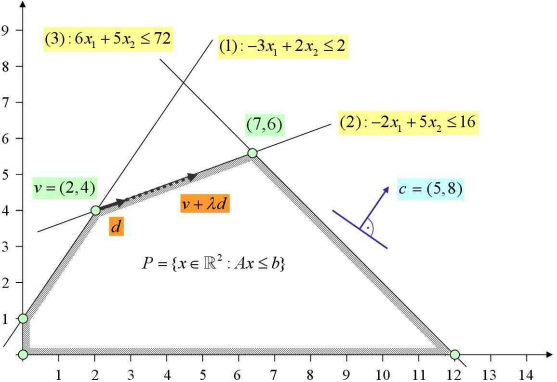
\includegraphics[width=9cm]{./Content/LinProg/simplex}
        \end{center}
  
        \begin{aufzaehlung}
          \item Basisinverse $\bar{A} = A_B^{-1}$ und evtl. zur Kontrolle Basislösung (= Eckpunkt) $v = \bar{A} b_B$ berechnen
          \item Reduzierte Kosten berechnen: $u = c \bar{A}$
          \item Wenn $u \geq 0$, dann Stopp!
          \item ($u \ngeq 0$). Wähle Spalte $j \in B$ in $u$ ($u_j < 0$) und berechne daraus 
            $d = - \bar{A}_j$, wobei $j$ in $\bar{A}_j$ die Spalte indiziert. $d$ entspricht der 
            Richtung, in der vom Eckpunkt weitergesucht wird.
          \item Stelle die Ungleichung $A v + \lambda A d \leq b$ mit $\lambda \in \mathbb{R}_0$ auf.
          \item Wenn $Ad \leq 0$, dann ist die grösste Zahl $\lambda$ welche obige Ungleichung erfüllt
            $\lambda^* = \infty$ und es muss gestoppt werden.
          \item ($0 \leq \lambda^* < \infty$). Berechne 
            $\lambda^* = \min \left\{ \frac{b_k - (Av)_k}{(Ad)_k} : k \in \{1,\ldots,m\}, (Ad)_k > 0 \right\}$,
            d.h. beachte nur Zeilen, wo $(Ad)_k > 0$ ist und berechne den Bruch; der kleinste Index $k$ 
            ist gesucht.
          \item Bilde neue zulässige Basisauswahl $B' = B - \{j\} \cup \{k\}$, wobei $j$ in die 
            Indizierung von der Basismatrix $A_B$ in der ursprünglichen $A$-Matrix zurückberechnet
            werden soll.
          \item Neuer Eckpunkt: $v' = v + \lambda^* d$
          \item Nächste Iteration mit $B = B'$ und $v = v'$ \ldots
        \end{aufzaehlung}
      \item Die Optimallösung: $f(v) = cv$
  \end{aufzaehlung}
  
\todo{Beispiel mit Zahlen!!!!!}